\subsubsection{Varying $c_L$ and $c_R$ while fixing $a_L = a_R = 1, b_L = b_R = 0$}

We start by examining this piecewise quadratic model with centered parabolas.
For this, we set $a_L = a_R = 1$ and $b_L = b_R = 0$ to keep the minimum in the center of the branches.
The parameters not fixed are $c_L$ and $c_R$.
They are both varied in the range $[0, 6]$, beyond that the behavior repeats, since $0 \equiv 6 \mod 6$.

This emulates the effect that $\chi_0$ has on branches $f_\A$ and $f_\C$.
Increasing $c_L$ increases the values on branches $f_\A$ and $f_\C$.
The effects of $E_0$ on branches $f_\B$ and $f_\D$ are lowering the value of the function at the left border of the branches and moving the minima on the branches to the left, as well as reducing the value of the function at the minima.
Decreasing $c_R$ does not have the same effects but rather lowers the values of the whole branches.

\Cref{fig:quadratic.full.2d.full} shows a 2D-scan of the periods of the stable cycles.
The structure in the middle left is enhanced and depicted in \Cref{fig:quadratic.full.2d.z1}.

A phenomenon like in the original model could not be found here.
But something very similar happens on the border of these wings.
\Cref{fig:quad.full.Cobwebs} shows the cobwebs along the line marked in \Cref{fig:quadratic.full.2d.z1}.
Before the border, there is one stable cycle with period 8.
This cycle is depicted in \Cref{fig:quad.full.CobwebA} and its symbolic sequence is $\A^3B\C^3\D$.
At the border, there is an area where two cycles coexist.
You cannot see this in the 2D scans above, since it only ever picks up on one cycle.
\Cref{fig:quad.full.CobwebB} shows the coexisting cycles at this border.
In contrast to the original model, the cycle that existed before in \Cref{fig:quad.full.CobwebA}, still exists alongside the new cycle with period 6.
The symbolic sequence of the new cycle is $\A^2\B\C^2\D$.

This is different from the dynamics in the original model in two ways.
First, the cycles before and after the area of coexistence have different periods.
And second, the cycles existing outside the area of coexistence still exist inside the area of coexistence.
In the original model, the cycles existing outside the area of coexistence would disappear at the border and new cycles would emerge inside this area.
Here, we simply observe two overlapping parameter regions which is something different from the original model.

\begin{figure}
	\centering
	\begin{subfigure}{0.4\textwidth}
		\centering
		\includegraphics[width=\textwidth]{21_Quadratic_mod6/2D_Period_Full/result.png}
		\caption{Full}
		\label{fig:quadratic.full.2d.full}
	\end{subfigure}
	\begin{subfigure}{0.4\textwidth}
		\centering
		\includegraphics[width=\textwidth]{21_Quadratic_mod6/2D_Period_Zoomed1/result.png}
		\caption{Zoomed}
		\label{fig:quadratic.full.2d.z1}
	\end{subfigure}
	\caption{2D Scan of Full Quadratic Model}
\end{figure}

\begin{figure}
	\centering
	\begin{subfigure}{0.3\textwidth}
		\centering
		\includegraphics[width=\textwidth]{21_Quadratic_mod6/Cobweb_A/result.png}
		\caption{Before border}
		\label{fig:quad.full.CobwebA}
	\end{subfigure}
	\begin{subfigure}{0.3\textwidth}
		\centering
		\includegraphics[width=\textwidth]{21_Quadratic_mod6/Cobweb_B/result.png}
		\caption{At border}
		\label{fig:quad.full.CobwebB}
	\end{subfigure}
	\begin{subfigure}{0.3\textwidth}
		\centering
		\includegraphics[width=\textwidth]{21_Quadratic_mod6/Cobweb_C/result.png}
		\caption{After border}
		\label{fig:quad.full.CobwebC}
	\end{subfigure}
	\caption{Cobwebs along marked line}
	\label{fig:quad.full.Cobwebs}
\end{figure}
